\section{Array addition and vectorization}

\textit{Task1} and \textit{Task2} ask for two functions, \texttt{routine1()} and \texttt{routine2()} respectively, to %
compute the element-wise sum of two float arrays, namely $a$ and $b$, into another array $c$. Both functions should also %
measure the time it takes the \texttt{for}-loop to complete. \\
The only difference between the two functions is that \texttt{routine2()} uses implicit parallelism. The actual %
logic remains the same. To avoid code duplication, I reused \texttt{routine1()} for both tasks and played with the compiler %
flags to achieve implicit parallelism.\\%
Source code \ref{code:array} shows the trivial implementation of the requested logic.\\
\begin{figure}[h!tb]
    \centering
    \captionsetup{type=plot}
    \caption{\label{plot:array}Run times by array size}
    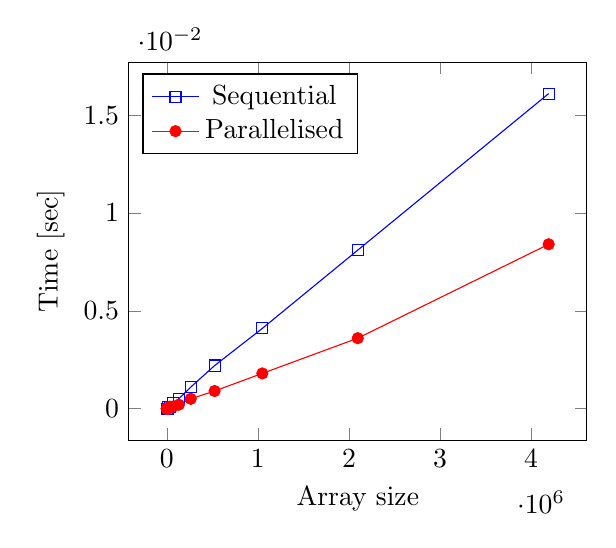
\begin{tikzpicture}
        \begin{axis}[
            title={},
            xlabel={Array size},
            ylabel={Time [sec]},
            legend pos=north west,
            grid style=dashed,
            width=7.4cm,
        ]
            \addplot[
                color=blue,
                mark=square,
                ]
                coordinates {
                    (16,0)
                    (32,0)
                    (64,0)
                    (128,0)
                    (256,0)
                    (512,0)
                    (1024,0)
                    (2048,0)
                    (4096,0)
                    (8192,0)
                    (16384,0.0001)
                    (32768,0.0001)
                    (65536,0.0003)
                    (131072,0.0005)
                    (262144,0.0011)
                    (524288,0.0022)
                    (1048576,0.0041)
                    (2097152,0.0081)
                    (4194304,0.0161)
                };
            
            \addplot[
                color=red,
                mark=*,
                ]
                coordinates {
                    (16,0)
                    (32,0)
                    (64,0)
                    (128,0)
                    (256,0)
                    (512,0)
                    (1024,0)
                    (2048,0)
                    (4096,0)
                    (8192,0)
                    (16384,0)
                    (32768,0.0001)
                    (65536,0.0001)
                    (131072,0.0002)
                    (262144,0.0005)
                    (524288,0.0009)
                    (1048576,0.0018)
                    (2097152,0.0036)
                    (4194304,0.0084)
                };
            \legend{Sequential, Parallelised}
        \end{axis}
    \end{tikzpicture}
\end{figure}%

After reading GCC's documentation\cite{GCC_vectorization, GCC_dev_opts, GCC_optimize_opts, GCC_x86_opts}, I decided %
to use the following commands to compile the code:
\begin{itemize}
    \item \textit{Task1} (Sequential version): \texttt{gcc -std=c99 -o bin/array-seq.out src/array.c}\\
        Arguments:
        \begin{itemize}
            \item[$\ast$] \texttt{-std=c99}: specifies the \textit{C} dialect used, \textit{C99} in this case. Needed to %
            allow index declarations inside \texttt{for}-loops. It does not impact speed and binary size whatsoever.
            \item[$\ast$] \texttt{-o bin/array-seq.out}: specifies the generated binary file path.
        \end{itemize}
    \item \textit{Task2} (Parallel version): \texttt{gcc -std=c99 -O2 -ftree-vectorize -funroll-loops %
        -fprefetch-loop-arrays -march=native -o bin/array-par.out src/array.c}\\
        Arguments:
        \begin{itemize}
            \item[$\ast$] \texttt{-std=c99}: specifies the \textit{C} dialect used, \textit{C99} in this case. Needed to %
            allow index declarations inside \texttt{for}-loops. It does not impact speed and binary size whatsoever.
            \item[$\ast$] \texttt{-O2}: applies general optimizations that do not involve a space-speed tradeoff%
                \cite{GCC_optimize_opts}
            \item[$\ast$] \texttt{-ftree-vectorize}: enables vectorization\cite{GCC_optimize_opts}
            \item[$\ast$] \texttt{-funroll-loops}: enables loop unrolling\cite{GCC_optimize_opts}
            \item[$\ast$] \texttt{-fprefetch-loop-arrays}: enables memory prefetching to aid looping on large arrays%
                \cite{GCC_optimize_opts}
            \item[$\ast$] \texttt{-march=native}: enables all supported extensions by the CPU in use\footnote{Useful %
                only if the compiling machine is the same as the executing one\cite{GCC_x86_opts}.}. It accelerates mathematical %
                operations, specifically floating-point ones, in hardware\cite{GCC_x86_opts}.
        \end{itemize}
\end{itemize}

The compilation flags, specifically those for the second version, were chosen after testing with multiple combinations. %
After weighting the obtained results, I decided to use the one that yielded a result correctly parallelized and had a visible %
increase in execution speed.\\
Alongside the plain \textit{C} code, I wrote a \textit{bash} script that wraps the compilation commands and binary execution %
into a single file to ease the testing phase. Each binary is called with array sizes between $2^4$ and $2^{22}$ (both inclusive) %
three times. Both sequential and parallelized runs dump their results into a \texttt{CSV} file so that I can examine %
them in external programs.%

\subsection*{Results analysis}
As per indication in the assignment, I executed the script on the University's cluster (GCC 4.8.5). Table %
\ref{table:array_seq_cluster} and Table \ref{table:array_par_cluster} report the obtained results.%

\begin{table}[h!tb]
    \centering
    \parbox{.45\linewidth}{
        \centering
\caption{Run times by array size - Sequential (times in seconds)}
\begin{tabular}{@{} c c c c c @{}}
\toprule
    \textbf{Size} & \textbf{Run 1}& \textbf{Run 2}& \textbf{Run 3}& \textbf{Average}\\
\midrule
    $2^4$ & 0.0000 & 0.0000 & 0.0000 & 0.0000\\
\lightrule
    $2^5$ & 0.0000 & 0.0000 & 0.0000 & 0.0000\\
\lightrule
    $2^6$ & 0.0000 & 0.0000 & 0.0000 & 0.0000\\
\lightrule
    $2^7$ & 0.0000 & 0.0000 & 0.0000 & 0.0000\\
\lightrule
    $2^8$ & 0.0000 & 0.0000 & 0.0000 & 0.0000\\
\lightrule
    $2^9$ & 0.0000 & 0.0000 & 0.0000 & 0.0000\\
\lightrule
    $2^{10}$ & 0.0000 & 0.0000 & 0.0000 & 0.0000\\
\lightrule
    $2^{11}$ & 0.0000 & 0.0000 & 0.0000 & 0.0000\\
\lightrule
    $2^{12}$ & 0.0000 & 0.0000 & 0.0000 & 0.0000\\
\lightrule
    $2^{13}$ & 0.0000 & 0.0000 & 0.0000 & 0.0000\\
\lightrule
    $2^{14}$ & 0.0000 & 0.0000 & 0.0000 & 0.0000\\
\lightrule
    $2^{15}$ & 0.0000 & 0.0000 & 0.0000 & 0.0000\\
\lightrule
    $2^{16}$ & 0.0000 & 0.0000 & 0.0000 & 0.0000\\
\lightrule
    $2^{17}$ & 0.0000 & 0.0000 & 0.0000 & 0.0000\\
\lightrule
    $2^{18}$ & 0.0000 & 0.0000 & 0.0000 & 0.0000\\
\lightrule
    $2^{19}$ & 0.0000 & 0.0000 & 0.0000 & 0.0000\\
\lightrule
    $2^{20}$ & 0.0200 & 0.0000 & 0.0200 & 0.0133\\
\lightrule
    $2^{21}$ & 0.0200 & 0.0000 & 0.0200 & 0.0133\\
\lightrule
    $2^{22}$ & 0.0200 & 0.0300 & 0.0300 & 0.0267\\
\bottomrule
\end{tabular}
\label{table:array_seq_cluster}
%
    }
    \parbox{.50\linewidth}{
        \input{assets/tables/array_par_cluster}%
    }
\end{table}

As is visible, the results are mostly instantaneous. Because zero values do not help in weighting the benefits of %
one version over the other, I opted to run the same script on my local machine, a laptop equipped with an Intel%
\textsuperscript{\textregistered} Core\textsuperscript{\texttrademark} i5-8300H at 2.30GHz and 16GB of RAM running Fedora %
38 (GCC 13.2.1). Table \ref{table:array_seq_local} and Table \ref{table:array_par_local} gather the obtained results.

\begin{table}[h!tb]
    \centering
    \parbox{.45\linewidth}{
        \centering
\caption{Run times by array size - Local machine - Sequential (times in seconds)}
\begin{tabular}{@{} c c c c c @{}}
\toprule
    \textbf{Size} & \textbf{Run 1}& \textbf{Run 2}& \textbf{Run 3}& \textbf{Average}\\
\midrule
    $2^4$ & 0.0000 & 0.0000 & 0.0000 & 0.0000\\
\lightrule
    $2^5$ & 0.0000 & 0.0000 & 0.0000 & 0.0000\\
\lightrule
    $2^6$ & 0.0000 & 0.0000 & 0.0000 & 0.0000\\
\lightrule
    $2^7$ & 0.0000 & 0.0000 & 0.0000 & 0.0000\\
\lightrule
    $2^8$ & 0.0000 & 0.0000 & 0.0000 & 0.0000\\
\lightrule
    $2^9$ & 0.0000 & 0.0000 & 0.0000 & 0.0000\\
\lightrule
    $2^{10}$ & 0.0000 & 0.0000 & 0.0000 & 0.0000\\
\lightrule
    $2^{11}$ & 0.0000 & 0.0000 & 0.0000 & 0.0000\\
\lightrule
    $2^{12}$ & 0.0000 & 0.0000 & 0.0000 & 0.0000\\
\lightrule
    $2^{13}$ & 0.0000 & 0.0000 & 0.0000 & 0.0000\\
\lightrule
    $2^{14}$ & 0.0001 & 0.0001 & 0.0001 & 0.0001\\
\lightrule
    $2^{15}$ & 0.0001 & 0.0001 & 0.0001 & 0.0001\\
\lightrule
    $2^{16}$ & 0.0003 & 0.0003 & 0.0002 & 0.0003\\
\lightrule
    $2^{17}$ & 0.0005 & 0.0005 & 0.0006 & 0.0005\\
\lightrule
    $2^{18}$ & 0.0010 & 0.0012 & 0.0010 & 0.0011\\
\lightrule
    $2^{19}$ & 0.0021 & 0.0021 & 0.0023 & 0.0022\\
\lightrule
    $2^{20}$ & 0.0041 & 0.0041 & 0.0041 & 0.0041\\
\lightrule
    $2^{21}$ & 0.0082 & 0.0081 & 0.0081 & 0.0081\\
\lightrule
    $2^{22}$ & 0.0163 & 0.0160 & 0.0161 & 0.0161\\
\bottomrule
\end{tabular}
\label{table:array_seq_local}
%
    }
    \parbox{.50\linewidth}{
        \centering
\caption{Run times by array size - Local machine - Parallelised (times in seconds)}
\begin{tabular}{@{} c c c c c @{}}
\toprule
    \textbf{Size} & \textbf{Run 1}& \textbf{Run 2}& \textbf{Run 3}& \textbf{Average}\\
\midrule
    $2^4$ & 0.0000 & 0.0000 & 0.0000 & 0.0000\\
\lightrule
    $2^5$ & 0.0000 & 0.0000 & 0.0000 & 0.0000\\
\lightrule
    $2^6$ & 0.0000 & 0.0000 & 0.0000 & 0.0000\\
\lightrule
    $2^7$ & 0.0000 & 0.0000 & 0.0000 & 0.0000\\
\lightrule
    $2^8$ & 0.0000 & 0.0000 & 0.0000 & 0.0000\\
\lightrule
    $2^9$ & 0.0000 & 0.0000 & 0.0000 & 0.0000\\
\lightrule
    $2^{10}$ & 0.0000 & 0.0000 & 0.0000 & 0.0000\\
\lightrule
    $2^{11}$ & 0.0000 & 0.0000 & 0.0000 & 0.0000\\
\lightrule
    $2^{12}$ & 0.0000 & 0.0000 & 0.0000 & 0.0000\\
\lightrule
    $2^{13}$ & 0.0000 & 0.0000 & 0.0000 & 0.0000\\
\lightrule
    $2^{14}$ & 0.0000 & 0.0000 & 0.0000 & 0.0000\\
\lightrule
    $2^{15}$ & 0.0001 & 0.0001 & 0.0001 & 0.0001\\
\lightrule
    $2^{16}$ & 0.0001 & 0.0001 & 0.0001 & 0.0001\\
\lightrule
    $2^{17}$ & 0.0003 & 0.0002 & 0.0002 & 0.0002\\
\lightrule
    $2^{18}$ & 0.0005 & 0.0006 & 0.0005 & 0.0005\\
\lightrule
    $2^{19}$ & 0.0009 & 0.0009 & 0.0009 & 0.0009\\
\lightrule
    $2^{20}$ & 0.0018 & 0.0018 & 0.0017 & 0.0018\\
\lightrule
    $2^{21}$ & 0.0036 & 0.0036 & 0.0036 & 0.0036\\
\lightrule
    $2^{22}$ & 0.0073 & 0.0082 & 0.0096 & 0.0084\\
\bottomrule
\end{tabular}
\label{table:array_par_local}
%
    }
\end{table}

Results from different machines with different architectures and components cannot be compared to each other, especially %
if the code is compiled for a particular machine. From now on, I am going to consider only the results obtained from my laptop.\\%
The average run times are plotted in Plot \ref{plot:array}. The obtained graph is the initial part of the so-called %
\textquote{Roofline model}. If the program were to be run with higher values and the machine was able to compute the result, 
the graph would rise to a certain point called \textquote{peak} and from then on would continue as a flat line having reached %
the maximum performance.\\%
Overall, by implicitly parallelizing the code, we gained around 57\% (average) more execution speed.%
\begin{figure}[h!tb]
    \centering
    \captionsetup{type=plot}
    \caption{\label{plot:array}Run times by array size}
    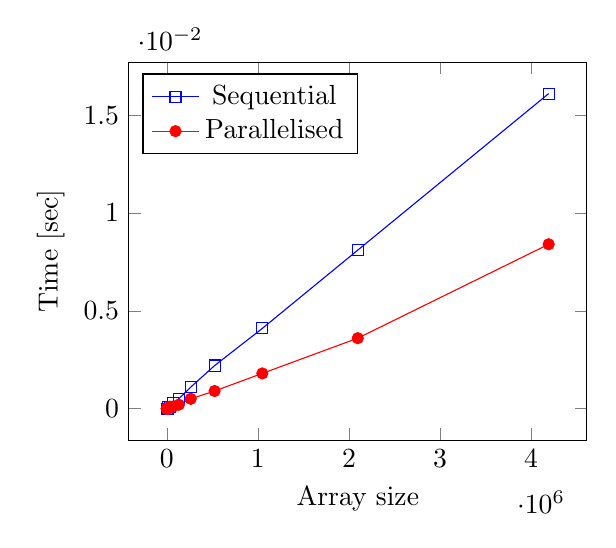
\begin{tikzpicture}
        \begin{axis}[
            title={},
            xlabel={Array size},
            ylabel={Time [sec]},
            legend pos=north west,
            grid style=dashed,
            width=7.4cm,
        ]
            \addplot[
                color=blue,
                mark=square,
                ]
                coordinates {
                    (16,0)
                    (32,0)
                    (64,0)
                    (128,0)
                    (256,0)
                    (512,0)
                    (1024,0)
                    (2048,0)
                    (4096,0)
                    (8192,0)
                    (16384,0.0001)
                    (32768,0.0001)
                    (65536,0.0003)
                    (131072,0.0005)
                    (262144,0.0011)
                    (524288,0.0022)
                    (1048576,0.0041)
                    (2097152,0.0081)
                    (4194304,0.0161)
                };
            
            \addplot[
                color=red,
                mark=*,
                ]
                coordinates {
                    (16,0)
                    (32,0)
                    (64,0)
                    (128,0)
                    (256,0)
                    (512,0)
                    (1024,0)
                    (2048,0)
                    (4096,0)
                    (8192,0)
                    (16384,0)
                    (32768,0.0001)
                    (65536,0.0001)
                    (131072,0.0002)
                    (262144,0.0005)
                    (524288,0.0009)
                    (1048576,0.0018)
                    (2097152,0.0036)
                    (4194304,0.0084)
                };
            \legend{Sequential, Parallelised}
        \end{axis}
    \end{tikzpicture}
\end{figure}